%%%% PROCESAR con PdfLaTeX !!!!!


\documentclass[12pt]{book}
\usepackage{geometry}\geometry{top=2cm,bottom=2cm,left=3cm,right=3cm}
\usepackage{amssymb}
\usepackage{amsmath}
\usepackage{graphicx}
\usepackage{txfonts}




\begin{document}
\thispagestyle{empty}

\vspace{3cm}
\begin {center}


\includegraphics[scale=.4]{descarga.jpeg}

\medskip
UNIVERSIDAD DE BUENOS AIRES

Facultad de Derecho

\vspace{3cm}


\textbf{\huge 	Trabajo Práctico Nº 2}
\\
\textbf{\huge Análisis Económico y Financiero}

\vspace{2cm}

\textbf{ECONOMÍA PRINCIPIOS Y APLICACIONES CUARTA EDICIÓN}
\\
\textbf{Mochón y Beker}
\\
\vspace{1cm}
\textbf{CAPÍTULO 2 - LA OFERTA, LA DEMANDA Y EL MERCADO: APLICACIONES}

\vspace{1cm}
Cátedra: Conesa
\\
1º cuat. 2020									            
\\
Comision 8610

\vspace{2cm}


\end {center}


\vspace{2cm}

\noindent Alumno:\,	Isaac Edgar Camacho Ocampo
 
\noindent Carrera:\,	Abogac\'ia

\vspace{1cm}

\noindent Buenos Aires, 2020


\tableofcontents

\chapter{CONCEPTOS BÁSICOS}
\section{El mercado}
Por mercado se entiende la institución social (que se corresponde o no con un lugar físico) en la cual los bienes y servicios, como así también los factores,se intercambian libre y voluntariamente.


\section{La Función de demanda}La función de demanda de un consumidor determinado para un bien concreto muestra la relación
existente entre la cantidad demandada de dicho bien y el precio de éste. La representación gráfica de la función de demanda es la curva de demanda, que evidencia la denominada ley de demanda.


\section{La función de oferta}La función de oferta muestra la relación existente entre el precio de un bien y las cantidades que un empresario desearía ofrecer de dicho bien. La curva de oferta es la representación gráfica de la función de oferta y refleja el comportamiento de los productores, que se concreta en que éstos aumentarán la cantidad lanzada al mercado si los precios aumentan.



\section{La curva de demanda}

\begin {center}
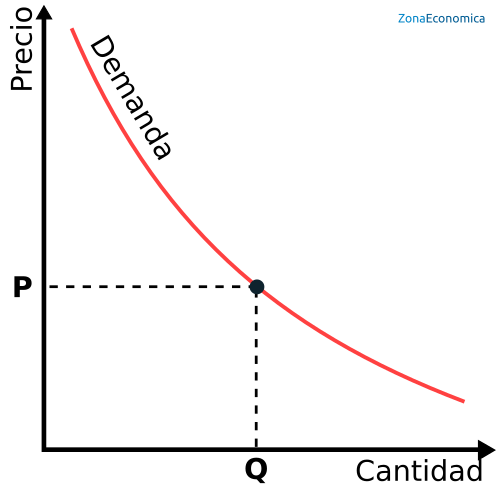
\includegraphics[scale=.7]{demanda_0.png}
\\
\begin{scriptsize}
La curva de demanda muestra la relacion inversamente proporcional que existe entre el precio y las cantidades demandadas, esto es que a mayor precio, la demanda disminuye, y a menor precio la demanda aumenta.

\end{scriptsize}\end{center}

La curva de demanda se desplazará cuando algunos de los siguientes factores experimenten una alteración:
\begin{itemize}
\item los ingresos de los consumidores,
\item los precios de los demás bienes relacionados, y
\item los gustos o preferencias.
\end{itemize}
Por el contrario, las variaciones del precio del bien demandado darán lugar a movimientos a lo largo de la curva de demanda.

\section{La curva de oferta}


\begin {center}
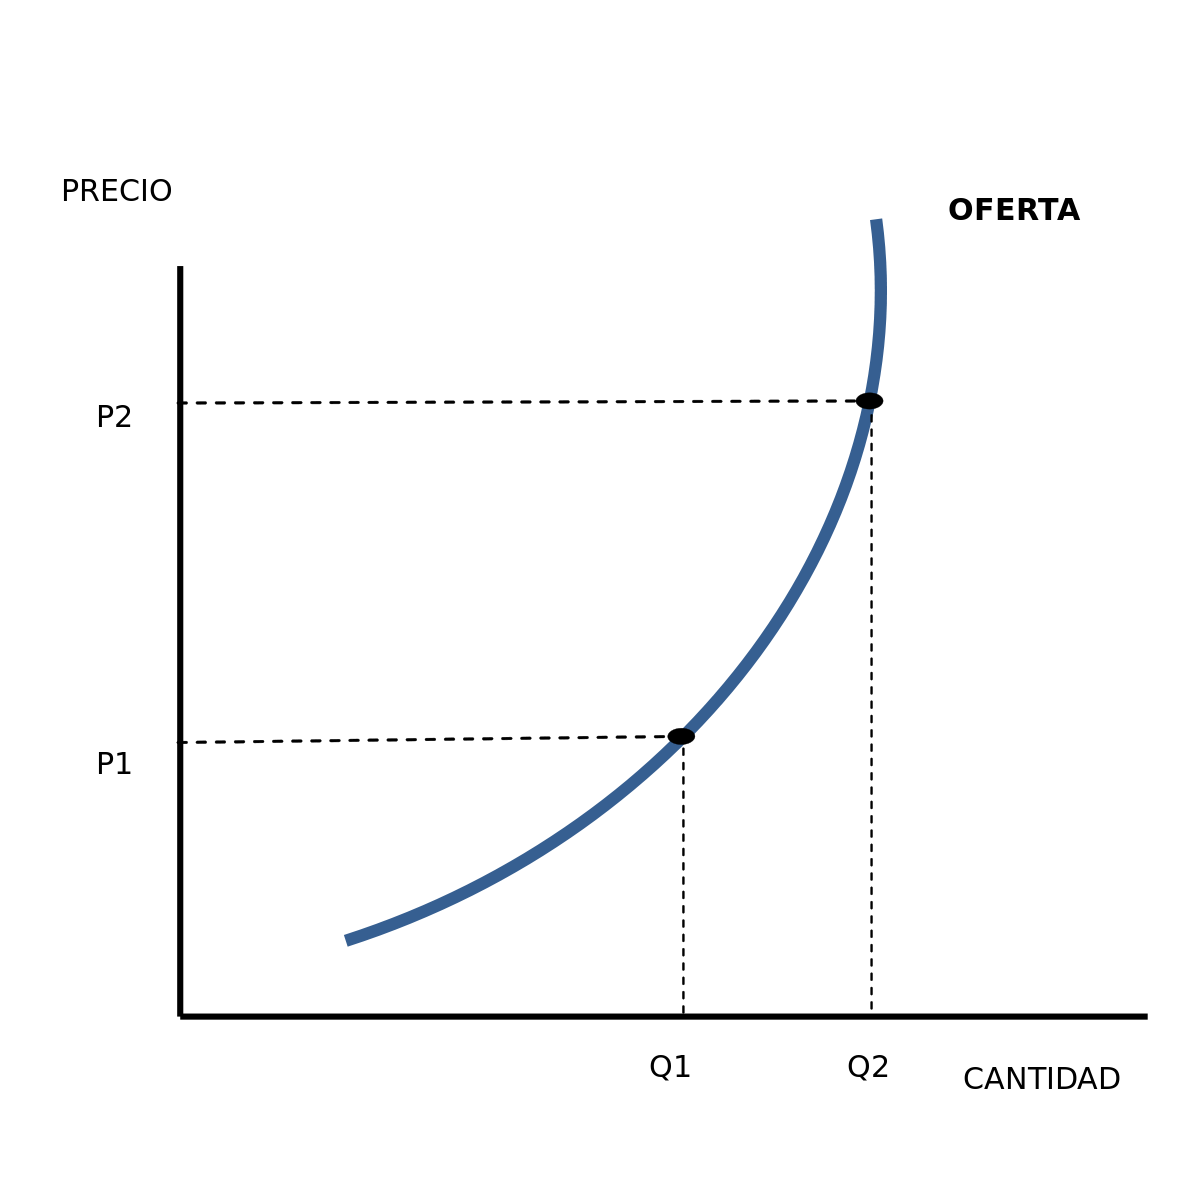
\includegraphics[scale=.2]{1200px-Curva_de_oferta.png}
\\
\begin{tiny}
La curva de oferta muestra la relacion directamente proporcional que existe entre el precio y las cantidades ofertadas, esto es que a mayor precio,oferta aumenta , y a menor precio la la oferta disminuye.

\end{tiny}\end{center}


Las variables más significativas que pueden originar desplazamientos de la curva de oferta son:

\begin{itemize}
\item el precio de los factores,
\item la tecnología y
\item los precios de los bienes relacionados.
\end{itemize}


\section{Equilibrio}

\begin {center}
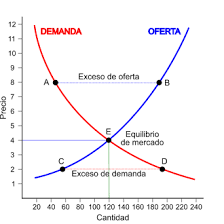
\includegraphics[scale=.7]{images.png}
\\
\textit{{\tiny El equilibrio se da en la interseccion de las curvas de oferta y demanda}}
\end{center}


En la situación de equilibrio se igualan las cantidades ofrecidas y demandadas. Un precio mayor que el de equilibrio producirá un exceso de oferta, esto es, una situación en la cual la cantidad ofrecida es superior a la demandada, mientras que si el precio es
menor se generará un exceso de demanda, es decir, una situación en la cual la cantidad demandada es superior a la cantidad ofrecida.


\section{El sistema de precios}
El sistema de precios es capaz, si se cumplen determinadas condiciones sobre el comportamiento de los agentes, de guiar la asignación de los recursos entre las diferentes industrias. La búsqueda de beneficios por parte de las empresas y el deseo de
los consumidores de aumentar su satisfacción por medio del consumo son dos elementos clave de este proceso.


\section{Precios máximos y mínimos }
La fijación de precios máximos o precios mínimos origina escasez o excedente en los mercados. 
Estos desequilibrios pueden permanecer indefinidamente.



\chapter{AUTOEVALUACIÓN}

\section{Preguntas de autoevaluaci\'on}
\begin{enumerate}

\item \textbf{¿Qué es un mercado?}
\\
\textbf{Rta:} El mercado de un producto está formado por todos los compradores y vendedores de ese producto.

\item \textbf{¿De qué factores depende la demanda de un bien?}
\\
\textbf{Rta:}
De los factores distintos del precio que desplazan la curva de demanda, los más importantes, son:
\begin{itemize}
\item Los ingresos de los consumidores.
\item Los precios de los bienes relacionados.
\item Los gustos o preferencias de los consumidores.
\item El tamaño del mercado o número de consumidores.
\end{itemize}


\item \textbf{¿Cuál es la diferencia entre las expresiones: demanda, cantidad de demanda, función de demanda, curva de demanda y ley de demanda?}
\\
\textbf{Rta:}
\begin{itemize}
\item \textbf{Demanda: }A las cantidades de un bien que los consumidores deseen y puedan comprar las denominamos demanda de dicho bien.
\item \textbf{Cantidad de demanda: }es la cantidad de un bien que los compradores quieren y pueden comprar.
\item \textbf{Función de demanda: }La función de demanda expresa la relación entre la cantidad demandada de un bien, su precio
y otras variables.
\item \textbf{Curva de demanda: }es la representación gráfica de la relación entre el precio de un bien y la cantidad demandada. Al trazar la curva de demanda, suponemos que se mantienen constantes los demás factores, excepto el precio, que puedan afectar la cantidad demandada.
\item \textbf{Ley de demanda:}La ley de la demanda se refiere a la relación inversa existente entre el precio de un bien y
la cantidad demandada, en el sentido de que al aumentar el precio disminuye la cantidad demandada, y lo contrario ocurre cuando se reduce el precio.
\end{itemize}

\item \textbf{¿De qué factores depende la oferta de un bien?}
\\
\textbf{Rta:}
\begin{itemize}
\item El precio de los factores productivos.
\item Los precios de los bienes relacionados. Precio del bien
\item La tecnología existente. Precio de los factores
\item El número de empresas oferentes.
\end{itemize}

\item \textbf{¿Cómo se forman los precios en los mercados?}
\\
\textbf{Rta:} El precio absoluto de un bien es su relación de cambio por dinero, esto es, el número de unidades monetarias que se necesitan para obtener a cambio una unidad del bien. El precio relativo de un bien es su precio en unidades de otro bien.

Los precios coordinan las decisiones de los productores y los consumidores en el mercado.
Precios bajos estimulan el consumo y desaniman la producción, mientras que precios altos tienden a reducir el consumo y estimulan la producción. Los precios actúan como el mecanismo equilibrador del mercado.

En la economía de mercado, las subas y bajas de precios, y la correspondiente aparición de beneficios y pérdidas, inducen a las empresas a producir eficientemente los bienes deseados.
Cuando el mecanismo de mercado funciona, el conjunto de mercados que integran la economía se equilibra alcanzando el equilibrio de mercado.
	

\item \textbf{¿En qué tipo de mercados se intercambian los siguientes bienes que llegan a los consumidores: naranjas, electricidad en su ciudad, acciones de Telefónica, revistas del corazón?}
\\
\textbf{Rta:}

\begin{itemize}
\item \textbf{naranjas: }mercados intervenidos
\item \textbf{electricidad en su ciudad: }mercados de competencia imperfecta
\item \textbf{acciones de Telefónica: }mercado competitivo
\item \textbf{revistas del corazón: }mercados transparentes,
\end{itemize}


\item \textbf{¿Qué ocurre cuando el precio de mercado al que se intercambia un bien es mayor que aquel que correspondería al equilibrio?}
\\
\textbf{Rta: }Para que un precio máximo sea relevante, debe ser inferior al precio de equilibrio.
genera una sobre oferta, ya que si el precio es mayor al de equilibrio esto provoca un incremento en la orefta, y una disminucion en la demanda.

\item \textbf{¿Por qué al bajar el precio de un bien las empresas están interesadas en ofrecer menos cantidad si para
ganar lo mismo deben vender más?}
\\
\textbf{Rta:} Es porque si baja el precio, el beneficio de la empresa es menor, la demanda de ese bien se incrementar\'a por la baja del precio pero la oferta disminuye, y los empresarios tendran menos interes de ofrecer ese bien porque el beneficio es bajo.

\item \textbf{¿Por qué el mismo bien puede ser inferior para un individuo y superior para otro?}
\\
\textbf{Rta:}
\textbf{Bien superior}. Bien cuya cantidad demandada aumenta al crecer el ingreso. Bien normal.
\\
\textbf{Bien inferior}. Bien cuya cantidad demandada disminuye cuando el ingreso aumenta.
\\
El mismo bien puede ser inferior para algunos individuos porque aumenta su ingreso y puede acceder a otros bienes que el considera superiores, y el mismo bien en cambio puede ser superior para otros individuos ya sera porque eran mas mas pobres y se les incremento el ingreso para poder acceder a dicho bien, o porque se disminuyo el ingreso de tal forma que es a lo que pueden aspirar.


\item \textbf{Si los precios son “señales”, cuando sube el precio de un bien, ¿quiere decir que debemos comprar más cantidad de ese bien cuanto antes?}
\\
\textbf{Rta:} Los mercados constituyen normalmente un buen mecanismo para organizar la actividad económica. Las economías de mercado aprovechan las fuerzas de la oferta y la demanda para asignar los recursos, en función de las señales que proporcionan los precios.
\\
Cuando sube el precio de un bien, no quiere decir que debemos comprar mas de ese bien, sino que algun factor productivo del bien esta en estado de escazes, lo que provoca que el precio se incremente.
\end{enumerate}

\chapter{EJERCICIOS Y APLICACIONES}
\section{Ejercicioss}
\begin{enumerate}
\item \textbf{1. Analice la siguiente información:}
\\
\begin{itemize}
\item Si se incrementa el precio de un bien sustitutivo del que estamos considerando, la curva de demanda del bien en cuestión se desplaza hacia la izquierda.
\\
\textbf{Rta: }Dos bienes serán sustitutivos si un aumento en el precio de uno motiva un desplazamiento hacia la
derecha en la curva de demanda del otro.


\item Es cierto que al aumentar los costos de producción, la curva de oferta de un bien se desplaza hacia la izquierda.
\textbf{Rta: }si, porque implica un incremento en los precios.
\item La diferencia entre una función genérica de demanda y una curva de demanda se debe a que:
\begin{enumerate}
\item la curva se representa en un gráfico, y la función, mediante una ecuación matemática.
\textbf{Rta: } corre\'cto !!!!
\item una curva de demanda es una función en la que todas las variables se mantienen constantes, a excepción del precio del bien.
\textbf{Rta: }Falso!!! una curva no es una funcion, sino que es un gr\'afico
\end{enumerate}
\end{itemize}



\item \textbf{Asistimos a la subasta de un cuadro. El precio de base ha sido de 80.000 pesos. Hay solo tres personas dispuestas a pagar este precio por el cuadro: el señor A, que como máximo pagaría 85.000 pesos; la señorita B, que está dispuesta a pagar como
máximo 90.000 pesos, y el señor C, que pagaría 93.000 pesos, pero no más.}
\begin{enumerate}
\item Señale los motivos por los que el precio de base no es el de equilibrio.
\textbf{Rta: }El precio de equilibrio, se da cuando la cantidad demandada es igual a la cantidad ofertada, por lo tanto si solo tres personas estan dispuesto a pagar el precio base, y consideramos que no son los u\'nicos seres humanos, habr\'ia otras personas que no estan dispuestas a pagar ese precio.
\item Indique un posible precio con el que acabará la subasta.
\textbf{Rta: }un precio ma\'ximo porque nadie pagar\'a mas.
\item Describa el papel del rematador.
\textbf{Rta: }asigna el recurso en funcion del precio, el rematador es el mercado, o la mano invisible de adam smith.
\end{enumerate}


\end{enumerate}


\end{document}
